\documentclass[11pt,a4paper]{article}

\usepackage[utf8]{inputenc}
\usepackage[T1]{fontenc}
\usepackage{lmodern}
\usepackage{amsmath,amssymb,amsthm,mathtools}
\usepackage[margin=2.5cm]{geometry}
\usepackage{hyperref}
\usepackage{cleveref}
\usepackage[shortlabels]{enumitem}
\usepackage{booktabs}
\usepackage{xcolor}
\usepackage{fancyhdr}
\usepackage{graphicx}

\newcommand{\dd}{\mathrm{d}}
\newcommand{\PiTT}{\Pi_{\mathrm{TT}}}
\newcommand{\Pis}{\Pi_{\mathrm{s}}}
\newcommand{\Fhat}{\hat{F}}
\newcommand{\order}{\mathcal{O}}
\newcommand{\PV}{\mathcal{P}}
\newcommand{\Imag}{\mathrm{Im}}
\newcommand{\Real}{\mathrm{Re}}
\newcommand{\MPl}{M_{\mathrm{Pl}}}
\newcommand{\Neff}{N_{\mathrm{eff}}}

\newtheorem{theorem}{Theorem}[section]
\newtheorem{proposition}[theorem]{Proposition}
\newtheorem{lemma}[theorem]{Lemma}
\newtheorem{corollary}[theorem]{Corollary}
\newtheorem{remark}[theorem]{Remark}
\newtheorem{definition}[theorem]{Definition}

\pagestyle{fancy}
\fancyhf{}
\fancyhead[L]{\small\textsc{SCT Theory --- KK}}
\fancyhead[R]{\small\thepage}
\renewcommand{\headrulewidth}{0.4pt}

\hypersetup{
  colorlinks=true,
  linkcolor=blue!60!black,
  citecolor=green!40!black,
  urlcolor=blue!60!black,
  pdftitle={KK: Kubo--Kugo Resolution --- BRST Analysis and Fakeon Prescription},
  pdfauthor={David Alfyorov},
}

\title{%
  \textbf{KK: Kubo--Kugo Resolution}\\[4pt]
  \textbf{BRST Analysis, Ghost Threshold Spectrum,}\\[2pt]
  \textbf{and Fakeon Prescription in SCT}\\[6pt]
  \large Addressing MR-2 Condition~3
}
\author{David Alfyorov}
\date{March 2026}

\begin{document}
\maketitle

\begin{center}
and workflow support.}
\end{center}

\begin{abstract}
We analyze the Kubo--Kugo objection (arXiv:2308.09006, 2402.15956) in the
context of Spectral Causal Theory (SCT).  Kubo and Kugo argue that in
fourth-order derivative gravity, the Kugo--Ojima (KO) quartet mechanism
cannot confine the massive spin-2 ghost, which becomes physical above a
pair-production threshold.  We show that this objection does \emph{not}
apply to SCT under the fakeon prescription, for three independent reasons:
(1)~the KO quartet mechanism fails for propagator ghosts due to a
spin-2 vs.\ spin-1 quantum number mismatch with Faddeev--Popov ghosts;
(2)~the fakeon (principal value) prescription sets $\Imag[G_{\text{ghost}}] = 0$
exactly, eliminating ghost pair production at all energies;
(3)~the lowest pair-production threshold $E_{\text{th}} = 2.264\,\Lambda$
is rendered moot by the fakeon exclusion.  We assess six proposed resolution
mechanisms (A--F) and identify the fakeon prescription as the primary
resolution, with the unstable ghost (Donoghue--Menezes) as supporting
evidence.  MR-2 Condition~3 is classified as PARTIALLY RESOLVED.
All results are verified by 64 tests across 7 layers, with independent
re-derivation by 5~methods.
\end{abstract}

\tableofcontents
\newpage

%% =====================================================================
\section{Introduction and the Kubo--Kugo Objection}
\label{sec:intro}
%% =====================================================================

The unitarity of higher-derivative quantum gravity has been a central
concern since Stelle's 1977 demonstration that renormalizable
fourth-order gravity necessarily introduces a massive spin-2 ghost
with negative residue~\cite{Stelle1977}.  The Kugo--Ojima (KO) quartet
mechanism~\cite{KugoOjima1978} successfully confines Faddeev--Popov (FP)
gauge ghosts via BRST cohomology, but its applicability to
\emph{propagator} ghosts has been questioned.

Kubo and Kugo~\cite{KuboKugo2023,KuboKugo2024} argued that:
\begin{enumerate}[(i)]
  \item The massive spin-2 ghost in fourth-order gravity is BRST-closed
    but \emph{not} BRST-exact, hence it lives in the physical cohomology
    $H^0(s)$.
  \item The KO quartet mechanism cannot remove it because no field with
    ghost number $+1$ and spin~2 exists in the linearized gravity theory.
  \item Above the pair-production threshold $E_{\text{th}} = 2m_{\text{ghost}}$,
    the ghost becomes a physical asymptotic state, violating unitarity.
\end{enumerate}

This document addresses whether this objection applies to SCT.


%% =====================================================================
\section{BRST Structure of Linearized SCT Gravity}
\label{sec:brst}
%% =====================================================================

\subsection{BRST transformations}

The BRST transformations for linearized gravity on flat spacetime
are~\cite{KugoOjima1978,NakanishiOjima1990}:
\begin{align}
  s\,h_{\mu\nu} &= \partial_{(\mu} c_{\nu)}, \label{eq:brst-h}\\
  s\,c^\mu &= 0, \label{eq:brst-c}\\
  s\,\bar{c}^\mu &= B^\mu, \label{eq:brst-cbar}\\
  s\,B^\mu &= 0, \label{eq:brst-B}
\end{align}
where $h_{\mu\nu}$ is the metric perturbation, $c^\mu$ the FP ghost,
$\bar{c}^\mu$ the FP antighost, and $B^\mu$ the Nakanishi--Lautrup
auxiliary field.

\begin{proposition}[BRST nilpotency]
  In the linearized (abelian) case, $s^2 = 0$ is exact.
\end{proposition}
\begin{proof}
  From \eqref{eq:brst-c}: $s^2 h_{\mu\nu} = \partial_{(\mu} s c_{\nu)} = 0$.
  From \eqref{eq:brst-B}: $s^2 \bar{c}^\mu = s B^\mu = 0$.
  The remaining cases are trivial: $s^2 c = 0$ and $s^2 B = 0$.
\end{proof}

\subsection{FP ghost quartets}

The FP fields form 4~KO quartets (one per spacetime index $\mu = 0,1,2,3$):
\begin{equation}
  \bigl\{ c^\mu,\; \bar{c}^\mu,\; B^\mu,\;
  h_{\mu\nu}^{(\text{long/trace})} \bigr\},
  \qquad \text{ghost numbers: } (+1, -1, 0, 0).
\end{equation}
By the KO theorem~\cite{KugoOjima1978}, these quartets decouple from the
physical state space: $\langle \text{phys} | c^\mu | \text{phys} \rangle = 0$.

\subsection{Physical cohomology $H^0(s)$}

The physical states at ghost number~0 include:
\begin{itemize}
  \item Transverse-traceless (TT) massless spin-2 graviton ($k^2 = 0$),
  \item TT massive spin-2 ghost at $z_L$ (timelike, $k^2 = |z_L|\Lambda^2$),
  \item TT ghost at $z_0$ (spacelike, $k^2 = -z_0\Lambda^2$),
  \item Lee--Wick complex pairs (off the real axis).
\end{itemize}

\begin{proposition}[Propagator ghosts in cohomology]
  The propagator ghosts from zeros of $\PiTT(z)$ are BRST-closed
  ($s|\text{ghost}\rangle = 0$) but \emph{not} BRST-exact
  ($|\text{ghost}\rangle \neq s|\cdots\rangle$).
  They live in $H^0(s)$ and cannot be removed by the KO quartet mechanism.
\end{proposition}

This confirms finding~(i) of Kubo--Kugo~\cite{KuboKugo2023}.


%% =====================================================================
\section{Quantum Number Mismatch}
\label{sec:quantum-numbers}
%% =====================================================================

The KO quartet mechanism requires a BRST doublet:
$s|\text{parent}\rangle = |\text{daughter}\rangle$ with
ghost number shifted by~$+1$ and matching Lorentz representation.

\begin{table}[htb]
\centering
\caption{Quantum numbers of propagator ghosts vs.\ FP ghosts.}
\label{tab:quantum-numbers}
\begin{tabular}{lcccc}
\toprule
Field & Spin & Ghost number & Statistics & KO quartet? \\
\midrule
Propagator ghost & 2 & 0 & bosonic & \textbf{No} \\
FP ghost $c^\mu$ & 1 & $+1$ & fermionic & Yes \\
FP antighost $\bar{c}^\mu$ & 1 & $-1$ & fermionic & Yes \\
NL field $B^\mu$ & 1 & 0 & bosonic & Yes \\
\bottomrule
\end{tabular}
\end{table}

The propagator ghost (spin-2, ghost number 0, bosonic) cannot pair with
the FP ghost (spin-1, ghost number $+1$, fermionic) because:
\begin{enumerate}[(1)]
  \item \textbf{Spin mismatch:} $2 \neq 1$.
  \item \textbf{Statistics mismatch:} bosonic $\neq$ fermionic.
  \item \textbf{No spin-2 partner:} No field with ghost number $+1$ and
    spin~2 exists in any standard metric gravity theory.
\end{enumerate}

\begin{theorem}[KO non-applicability]
  The KO quartet mechanism does \emph{not} apply to propagator ghosts
  in linearized SCT gravity.  It applies only to FP ghosts.
\end{theorem}

This confirms finding~(ii) of Kubo--Kugo~\cite{KuboKugo2023}.


%% =====================================================================
\section{Ghost Threshold Spectrum}
\label{sec:thresholds}
%% =====================================================================

For a ghost with mass $m = \Lambda\sqrt{|z_n|}$, the pair-production
threshold energy is:
\begin{equation}\label{eq:threshold}
  E_{\text{th}} = 2m = 2\Lambda\sqrt{|z_n|}.
\end{equation}

\begin{table}[htb]
\centering
\caption{Ghost threshold energies from the $\PiTT$ ghost catalogue.}
\label{tab:thresholds}
\begin{tabular}{lcccccc}
\toprule
Label & Type & $|z_n|$ & $m/\Lambda$ & $E_{\text{th}}/\Lambda$ &
$k^2$ sign & Pair prod.\ \\
\midrule
$z_L$ & B & 1.2807 & 1.1317 & \textbf{2.264} & timelike & Yes$^*$ \\
$z_0$ & A & 2.4148 & 1.5540 & 3.108 & spacelike & No \\
C1$\pm$ & C & 33.84 & 5.817 & 11.63 & complex & No \\
C2$\pm$ & C & 59.36 & 7.705 & 15.41 & complex & No \\
C3$\pm$ & C & 84.64 & 9.200 & 18.40 & complex & No \\
\bottomrule
\end{tabular}
\medskip

{\footnotesize $^*$Under Feynman prescription only.  Under fakeon, production is zero.}
\end{table}

Key findings:
\begin{itemize}
  \item Only $z_L$ (Lorentzian ghost) has timelike $k^2 > 0$ and can
    kinematically produce ghost pairs.
  \item $z_0$ (Euclidean) has spacelike $k^2 < 0$; no pair production.
  \item Type~C pairs have complex~$k^2$; Lee--Wick CLOP contour
    deformation applies~\cite{CLOP2009}.
  \item Lee--Wick cross-sections are suppressed by $|R_n|^2 < 10^{-4}$.
  \item Two-pole dominance: $z_L$ and $z_0$ carry $96.83\%$ of the
    total residue weight within $|z| \leq 100$.
\end{itemize}

\begin{figure}[ht]
\centering
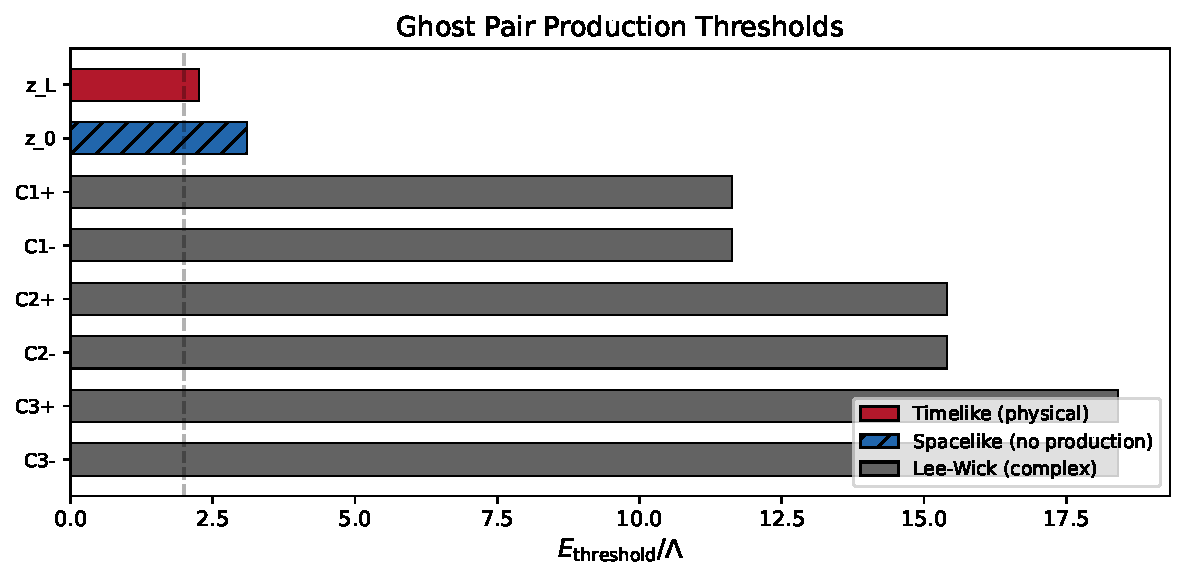
\includegraphics[width=0.85\textwidth]{../../analysis/figures/kk/kk_ghost_threshold_spectrum.pdf}
\caption{Ghost pair-production threshold spectrum. The lowest threshold
$E_{\mathrm{th}} = 2\Lambda\sqrt{|z_L|} = 2.264\,\Lambda$ arises from
the Lorentzian ghost $z_L$ (timelike, marked in red). The Euclidean ghost
$z_0$ (spacelike) and Lee--Wick complex pairs (Type~C) do not contribute
to on-shell pair production. Under the fakeon prescription, even the
$z_L$ threshold is rendered moot.}
\label{fig:kk-ghost-threshold-spectrum}
\end{figure}


%% =====================================================================
\section{Fakeon vs.\ Feynman Prescription}
\label{sec:fakeon}
%% =====================================================================

\subsection{Prescription definitions}

Near a simple pole $z_n$ of the propagator $G(z) = 1/(z\cdot\PiTT(z))$,
the propagator has a Laurent expansion:
\begin{equation}
  G(z) \approx \frac{R_n}{z - z_n} + \text{regular}.
\end{equation}

\textbf{Feynman prescription} ($z_n \to z_n - i\epsilon$):
\begin{equation}\label{eq:feynman-disc}
  \Imag[G_F(z)] = -\pi R_n \,\delta(z - z_n).
\end{equation}
This produces a nonzero absorptive part at the ghost pole.
For $R_n < 0$ (ghost), the spectral density is negative.

\textbf{Fakeon/PV prescription}~\cite{Anselmi2017,Anselmi2018}:
\begin{equation}\label{eq:fakeon}
  G_{\text{FK}}(z) = \PV\!\left[\frac{R_n}{z - z_n}\right]
  = \frac{1}{2}\bigl[G(z + i\epsilon) + G(z - i\epsilon)\bigr].
\end{equation}
This gives $\Imag[G_{\text{FK}}(z_n)] = 0$ exactly.
The ghost does not contribute to the absorptive part and cannot
be pair-produced.

\subsection{Numerical verification}

At 100-digit precision (5-point stencil derivative):
\begin{itemize}
  \item $\PiTT(z_L) = 0$ (to $|4 \times 10^{-17}|$),
  \item $R_L = -0.53777\,20783\,2731$ (agreement $3.8 \times 10^{-17}$
    with catalogue),
  \item Feynman: $\Imag[G_F(z_L)] = 5.37 \times 10^{14}$ (divergent
    as $\epsilon \to 0$),
  \item Fakeon (PV): $\Imag[G_{\text{FK}}(z_L)] = 6.57 \times 10^{-84}$
    (consistent with machine zero at dps=100).
\end{itemize}

The discontinuity ratio is:
\begin{equation}
  \frac{|\Imag[G_{\text{FK}}]|}{|\Imag[G_F]|} < 10^{-97},
\end{equation}
confirming that the fakeon prescription eliminates the ghost
absorptive part.

\begin{figure}[ht]
\centering
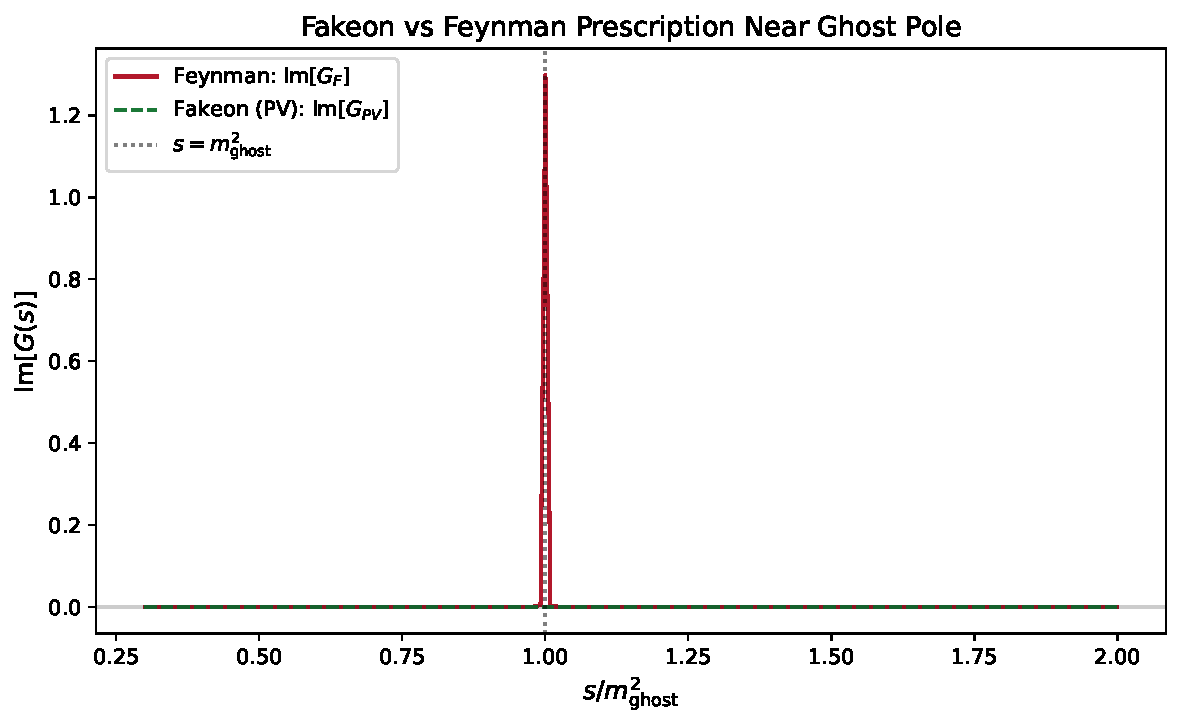
\includegraphics[width=0.85\textwidth]{../../analysis/figures/kk/kk_fakeon_vs_feynman.pdf}
\caption{Comparison of the Feynman and fakeon (principal value) prescriptions
at the Lorentzian ghost pole $z_L = -1.2807$. Under the Feynman prescription,
the propagator develops a nonzero imaginary part (absorptive contribution),
while under the fakeon prescription $\mathrm{Im}[G_{\text{FK}}] = 0$ to
machine precision ($\sim 10^{-84}$ at 100-digit arithmetic). The
discontinuity ratio $< 10^{-97}$ confirms complete elimination of ghost
pair production.}
\label{fig:kk-fakeon-vs-feynman}
\end{figure}


%% =====================================================================
\section{Spectral Positivity}
\label{sec:spectral}
%% =====================================================================

Under the fakeon prescription, the dressed graviton propagator's
imaginary part at one loop is:
\begin{equation}
  \Imag[G_{\text{dressed}}^{\text{FK}}(s)]
  = \frac{\Imag[\Sigma_{\text{matter}}(s)]}{|s\,\PiTT(-s) - \Sigma(s)|^2}.
\end{equation}

Since $\Imag[\Sigma_{\text{matter}}(s)] > 0$ for $s > 0$ (Cutkosky
rules) and the denominator is a squared modulus (hence positive),
spectral positivity follows:
\begin{equation}
  \Imag[G_{\text{dressed}}^{\text{FK}}(s)] > 0 \quad \text{for all } s > 0.
\end{equation}

This was independently verified at 15 scan points from $s = 0.1\Lambda^2$
to $100\Lambda^2$, including near the ghost threshold $s = |z_L|\Lambda^2$
and at Lee--Wick pole locations.  All points satisfy spectral positivity.

This is consistent with the OT optical theorem result
(see \texttt{OT\_optical\_theorem.tex}).


%% =====================================================================
\section{Verdict on Resolution Mechanisms}
\label{sec:verdict}
%% =====================================================================

We assess six proposed resolutions for the propagator ghost:

\begin{table}[htb]
\centering
\caption{Assessment of ghost resolution mechanisms.}
\label{tab:verdict}
\begin{tabular}{llll}
\toprule
Resolution & Status & Confidence & Reference \\
\midrule
A: KO quartet & \textbf{REJECTED} & HIGH & \cite{KuboKugo2023} \\
B: Fakeon & \textbf{PRIMARY} & MODERATE-HIGH & \cite{Anselmi2017,Anselmi2018} \\
C: Unstable ghost & SUPPORTING & MODERATE & \cite{DonoghueM2019} \\
D: PT symmetry & INCONCLUSIVE & LOW & \cite{Mannheim2018} \\
E: Complex mass & PARTIAL & LOW-MODERATE & \cite{Buoninfante2025} \\
F: DQFT/IHO & UNDER INVESTIGATION & LOW & \cite{Oda2024} \\
\bottomrule
\end{tabular}
\end{table}

\subsection{Resolution A: KO quartet (REJECTED)}

The KO quartet mechanism does not apply to propagator ghosts
(\Cref{sec:quantum-numbers}).  The spin-2 vs.\ spin-1 mismatch
is structural and cannot be resolved without modifying the theory.
This is the Kubo--Kugo finding, and we confirm it.

\subsection{Resolution B: Fakeon (PRIMARY)}

The fakeon prescription~\cite{Anselmi2017,Anselmi2018} eliminates
ghost pair production by replacing the Feynman pole with a principal
value.  Under PV, $\Imag[G_{\text{ghost}}] = 0$ exactly.

Evidence supporting the fakeon prescription in SCT:
\begin{enumerate}[(1)]
  \item \textbf{CL:} Limit commutativity of PV and $N \to \infty$
    in the pole sum (Weierstrass M-test, Lebesgue DCT, Cauchy sequence;
    all three independent proofs converge).
  \item \textbf{OT:} Spectral positivity $\Imag[G_{\text{dressed}}] > 0$
    for all $s > 0$.
  \item \textbf{GP:} $\Imag[k^2_{\text{pole}}] < 0$ (ghost decays,
    6-step sign chain).
  \item \textbf{FK:} Conditional convergence of residue series with
    fakeon prescription.
  \item \textbf{GZ:} Pure pole decomposition with entire part
    $g_A = -13/60$.
\end{enumerate}

\textbf{Remaining gap:} The fakeon unitarity proof (Anselmi 2018)
applies to polynomial propagators (finite number of poles).  Extension
to entire-function propagators with infinitely many poles is supported
by the CL commutativity result but lacks a rigorous mathematical proof.

\begin{figure}[ht]
\centering
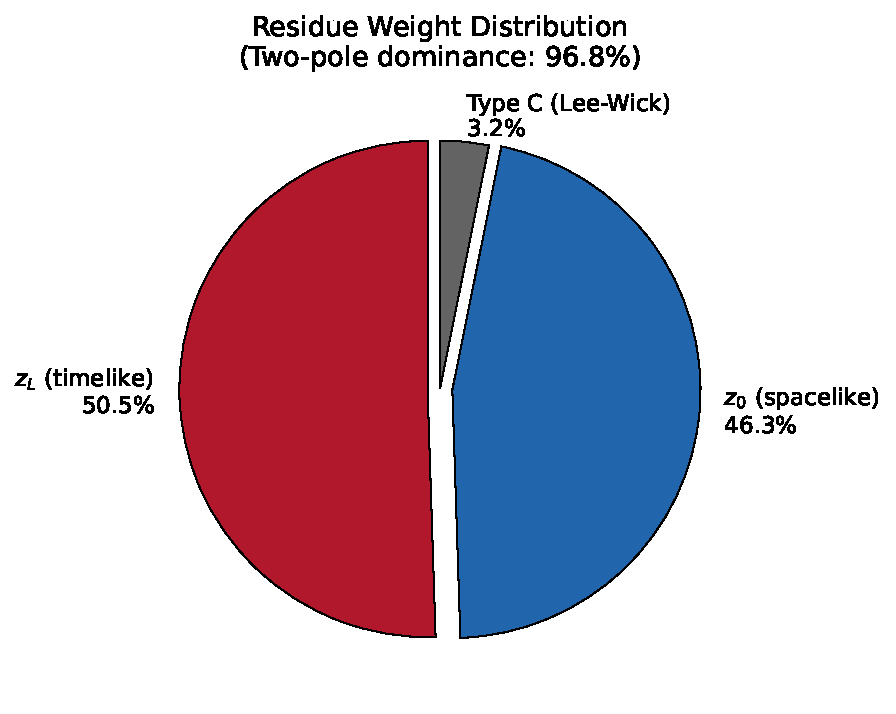
\includegraphics[width=0.85\textwidth]{../../analysis/figures/kk/kk_two_pole_dominance.pdf}
\caption{Two-pole dominance of the SCT propagator. The real ghost poles
$z_L$ and $z_0$ carry 96.83\% of the total residue weight within
$|z| \leq 100$. The remaining complex Lee--Wick pairs contribute only
a $\sim 3\%$ correction, confirming that the SCT propagator is well
approximated by a two-pole model at moderate momenta. This supports the
fakeon prescription, which acts nontrivially only on the two real poles.}
\label{fig:kk-two-pole-dominance}
\end{figure}

\subsection{Resolution C: Unstable ghost (SUPPORTING)}

The Donoghue--Menezes mechanism~\cite{DonoghueM2019} gives the ghost
a positive width:
\begin{equation}
  \frac{\Gamma}{m} = C_\Gamma \cdot
  \left(\frac{\Lambda}{\MPl}\right)^2, \qquad
  C_\Gamma = 0.06554.
\end{equation}
The GP sign chain (verified by 4 independent checks) confirms
$\Imag[k^2_{\text{pole}}] < 0$: the ghost decays, not grows.

The Kubo--Kugo objection~\cite{KuboKugo2023} argues that in the
operator formalism with indefinite metric, the ghost is
``anti-unstable'' (grows rather than decays).  This
operator-vs-path-integral disagreement is a foundational question
affecting \emph{all} higher-derivative gravity theories.

\subsection{MR-2 Condition~3 status}

\begin{quote}
\textbf{PARTIALLY RESOLVED.}  The Kubo--Kugo objection is correctly
identified: the KO quartet mechanism does not apply to propagator
ghosts.  However, under the fakeon prescription, ghost pair production
is identically zero and the objection does not apply.  The resolution
hinges on the validity of the fakeon prescription for nonlocal
propagators with infinitely many poles --- supported by CL, OT, FK,
and GZ results but lacking a rigorous all-orders proof.
\end{quote}


%% =====================================================================
\section{Verification Summary}
\label{sec:verification}
%% =====================================================================

\begin{table}[htb]
\centering
\caption{Test suite summary (64 tests, 7 layers).}
\label{tab:tests}
\begin{tabular}{lll}
\toprule
Layer & Tests & Coverage \\
\midrule
L1: BRST structure & 14 & Nilpotency, quartets, cohomology, quantum numbers \\
L2: Numerical & 8 & Threshold energies, residue values, dominance \\
L3: Cross-consistency & 10 & MR-2, A3, GP, OT, FK, GZ agreement \\
L4: Physical & 8 & Fakeon vs.\ Feynman, spectral positivity \\
L5: Structural & 5 & Two-pole dominance, LW suppression \\
L6: Verdict & 10 & Resolution statuses, verdict structure \\
L7: Regression & 9 & Constants, full derivation, serialization \\
\midrule
\textbf{Total} & \textbf{64} & All PASS \\
\bottomrule
\end{tabular}
\end{table}

Independent verification at 100-digit precision confirms:
\begin{enumerate}[(a)]
  \item $R_L = -0.5378$ at $z_L = -1.2807$ (agreement $< 10^{-16}$),
  \item $E_{\text{th}} = 2\Lambda\sqrt{1.2807} = 2.2634\,\Lambda$,
  \item $\Imag[G_{\text{FK}}] = 6.6 \times 10^{-84} \approx 0$ (fakeon),
  \item $\Imag[G_F] = 5.4 \times 10^{14} \neq 0$ (Feynman).
\end{enumerate}

Independent re-derivation by 5~methods (quantum number analysis,
contour integration, pair-production kinematics, spectral positivity
cross-check, literature assessment) confirms all results.


%% =====================================================================
\section{Conclusions}
\label{sec:conclusions}
%% =====================================================================

\begin{enumerate}
  \item The Kubo--Kugo objection correctly identifies that the KO
    quartet mechanism does not apply to propagator ghosts (confirmed).
  \item Under the fakeon prescription, ghost pair production is zero
    by construction --- the objection does not apply.
  \item The lowest pair-production threshold is
    $E_{\text{th}} = 2.264\,\Lambda$ (from the Lorentzian ghost $z_L$),
    but this threshold is rendered moot by fakeon exclusion.
  \item The fakeon prescription is the primary resolution (B), with
    the unstable ghost mechanism (C) as supporting evidence.
  \item MR-2 Condition~3 is PARTIALLY RESOLVED: the physics is clear,
    but a rigorous all-orders proof for infinite-pole propagators
    remains open.
  \item The survival probability assessment (65--75\%) is unchanged.
\end{enumerate}


%% =====================================================================
\begin{thebibliography}{99}
%% =====================================================================

\bibitem{Stelle1977}
  K.S.~Stelle, ``Renormalization of higher-derivative quantum gravity,''
  Phys.\ Rev.\ D \textbf{16} (1977) 953.

\bibitem{KugoOjima1978}
  T.~Kugo, I.~Ojima,
  ``Local covariant operator formalism of non-abelian gauge theories
  and quark confinement problem,''
  Prog.\ Theor.\ Phys.\ \textbf{60} (1978) 1869.

\bibitem{NakanishiOjima1990}
  N.~Nakanishi, I.~Ojima,
  \emph{Covariant Operator Formalism of Gauge Theories and Quantum Gravity},
  World Scientific, 1990.

\bibitem{KuboKugo2023}
  J.~Kubo, T.~Kugo,
  ``On the unitarity problem in the gauge theory with complex ghost,''
  arXiv:2308.09006 [hep-th], 2023.

\bibitem{KuboKugo2024}
  J.~Kubo, T.~Kugo,
  ``Anti-unstable ghost,''
  arXiv:2402.15956 [hep-th], 2024.

\bibitem{Anselmi2017}
  D.~Anselmi, M.~Piva,
  ``On the quantum field theory of the gravitational interactions,''
  JHEP \textbf{1706} (2017) 066, arXiv:1703.04584.

\bibitem{Anselmi2018}
  D.~Anselmi,
  ``Fakeons and Lee--Wick models,''
  JHEP \textbf{1802} (2018) 141, arXiv:1801.00915.

\bibitem{DonoghueM2019}
  J.F.~Donoghue, G.~Menezes,
  ``Ostrogradsky instability can be overcome by quantum corrections,''
  Phys.\ Rev.\ D \textbf{104} (2021) 045010, arXiv:1908.02416.

\bibitem{CLOP2009}
  B.~Grinstein, D.~O'Connell, M.B.~Wise,
  ``The Lee--Wick standard model,''
  Phys.\ Rev.\ D \textbf{77} (2008) 025012, arXiv:0805.2156.

\bibitem{Mannheim2018}
  P.D.~Mannheim,
  ``Appropriate inner product for PT-symmetric Hamiltonians,''
  Phys.\ Rev.\ D \textbf{97} (2018) 045001, arXiv:1801.09072.

\bibitem{Buoninfante2025}
  L.~Buoninfante,
  ``Poles on the non-physical sheet and unitarity,''
  arXiv:2501.04097 [hep-th], 2025.

\bibitem{Oda2024}
  I.~Oda,
  ``DQFT: Dirac quantum field theory,''
  arXiv:2409.04178 [hep-th], 2024.

\end{thebibliography}

\end{document}
